% \title{Measurement: Errors and Error Analysis}
% \author{An Introduction to Physics through Experiments}
% \date{}
% \maketitle

\chapter{Sensitivity to Errors in Measurement and Preliminary Error Analysis}

\section{Objectives}

\begin{enumerate}
    \item To recognise different kinds of errors, in particular systematic errors, errors due to the least count of an instrument, random errors, and errors in time measurement.
    \item To learn to use Vernier calipers and the screw gauge.
    \item To begin to understand propagation of errors. 
    \item To use preemptive error analysis to plan an experiment. 
    
    %\item To study the propagation of errors from measured to derived quantities.
\end{enumerate}

\section{Introduction}

When observing the time period of the simple pendulum, you already became aware of the extent to which you are certain of your time measurement. In fact, all the measurements you made -- of mass, of length, of time -- were uncertain. In experimental physics it is of enormous importance to understand how different kinds of errors arise, because without an understanding of errors it is difficult to make sense of your data. This is a vast and subtle subject, and so you will learn the elements of it slowly.

It is important to appreciate that in physics \textit{an error is not a mistake}. An error in physics is a measure of how certain (and therefore how uncertain!) we are of a measurement. All measurements are to a greater or smaller extent uncertain; there is no such thing as a perfect measurement: therefore, there is no such thing as an error-free measurement. 

To broaden the scope or your understanding of errors, you will use not only the data you got while observing the oscillations of a pendulum, you will also learn to use two very useful instruments, the Vernier calipers and the screw gauge, which highlight beautifully certain kinds of errors.

\begin{tip}
Example: if you use a metre scale with a least count (smallest division) of $0.1 cm$ upside down to measure a pencil and misread the scale as $94.6 cm$ instead of $5.4 cm$, this is a \textbf{mistake}.\\

However, if you note down the length as being $5.4 cm$, but rightly note that it is not \textbf{exactly} $5.4 cm$, but simply that your measuring device does not allow for any more precision, this is a measure of \textbf{uncertainty}. \\

We will expect you to have verified that you haven't done the former, and will take for granted from here on that no mistakes were made in the collection of data.
\end{tip}

The complete statement of a measured value \textit{must} include an estimate of the level of confidence associated with the value. This allows people to judge the quality of the experiment and allows for comparisons with other similar estimates of the same quantity, or theoretical prediction.  

\begin{imp}
A proper experiment must report both a ``best'' value and an uncertainty for each measured quantity. You will be expected to do this in all your experiments. 
\end{imp}

Without an uncertainty estimate, it is impossible to answer the basic scientific question: Does my result agree with a theoretical prediction or results from other experiments? This question is fundamental for deciding if a scientific hypothesis is confirmed or refuted.

\section{Systematic Errors} 

Suppose that you are weighing yourself and the pointer is at 1 $kg$ even when no-one is standing on the scales. Then, obviously, all measurements will differ from the correct weights by 1 $kg$. Such an error is called \text{systematic}, since it appears systematically in all readings. The only way to eliminate a systematic error is to identify its cause and eliminate that. Some devices allow such checking to be done relatively easily, e.g. a metre scale or a weighing scale, but many others do not, e.g. electrical devices with internal errors. Estimating possible errors due to such systematic effects will depend on your understanding of your apparatus and the skill you have developed for thinking about possible problems.  However, if you get a value for some quantity that seems rather far off what you expect, you should think about such possible sources more carefully. You could end up trusting a device that you do not know is faulty. This happens very often, to the best of us. 

\begin{question}
\paragraph{Question:} You use a ruler whose end is worn out, so that it effectively begins at 2 $mm$. How can you avoid the systematic error that would arise if you used the ruler naively?~\\

%\vspace{0.5 cm}

\paragraph{Question:} A systematic error can be either positive or negative. What is the difference and under what circumstances would they arise? (If you don't understand this point, you may end up doubling a systematic error in trying to eliminate it.)
\end{question}

\subsection{Least-count-related Errors}

When you make a length measurement with a ruler whose smallest division is 1 $mm$ in size. If you imagine aligning an object of a certain length against a ruler, you can ensure that one end of the object is flush with a mark on the ruler but you cannot ensure that the other end is also flush with another mark -- it general it will be somewhere between two successive marks, and you cannot tell exactly where it is; normally the best that you can do is say, ``It's more than halfway between'', or ``It's less than halfway between''. So the error associated with the least count of the instrument is normally between half and one full least count. 

Because the least count of an instrument is a limitation, one can try to subdivide the region between two marks. It is obvious, however, that this is not going to work beyond a point, since we will simply not be able to tell where the end of the object lies. 

So a couple of clever designs \textit{effectively} sub-divide the region. The most beautiful of these designs was first included in an instrument called Vernier calipers; another design is found in the screw gauge. You will learn how to use both of these instruments. (The essential design of the Vernier calipers is incorporated in many other instruments, and we then speak of it as having a Vernier scale.)

\section{Vernier Calipers and the Screw Gauge}

\subsection{Vernier Calipers}

You will regularly come across vernier scales in the lab when using calipers, angular vernier scales (in spectrometers), and travelling microscopes. Vernier scales allow you to read off a value more precisely than when using an ordinary scale. In this section, we will explain how this works.

First consider a ``main scale'' with a least count of 1 unit (you could imagine this is $1mm$, if you wish). This implies that any distance between, say, the 2 and 3 unit marks cannot be determined accurately. In other words, the best you could say is that an object is ``2 and a bit'' units. The vernier scale allows you to \textbf{quantify} this ``bit'' to some extent.  

The method is ingenious: instead of measuring this ``bit'' directly, its magnitude is translated into a a degree of coincidence between two scales, the main scale and a secondary one called the Vernier scale. The Vernier scale has divisions that are \textbf{slightly} smaller than that of the main scale, such that $n$ divisions on the Vernier scale have the same length as $n-1$ divisions of the main scale. For example,  9 divisions on the main scale may coincide with 10 divisions on the Vernier scale (see Figure (\ref{fig:vernier_1})). 

\begin{figure}[!htb]
    \centering
    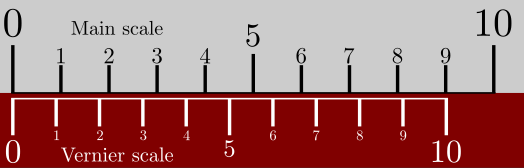
\includegraphics[scale=0.75]{figs/vernier1.png}
    \caption{10 vernier scale divisions are set to coincide with 9 main scale divisions.}
    \label{fig:vernier_1}
\end{figure}

\begin{question}
    \paragraph{Question:} What is the spacing between two vernier scale divisions? Is it:
    \begin{enumerate}
        \item 1 unit?
        \item 0.1 units?
        \item 0.9 units?
    \end{enumerate}
\end{question}

Let us now try to measure the smallest possible distance between 0 and 1 unit. Take a set of Vernier calipers and close the jaws completely. If there is no zero-error, the only two readings on the vernier scale and main scale that match are the $0$ and $10$.

\begin{figure}[!htb]
        \begin{subfigure}[b]{0.5\textwidth}
                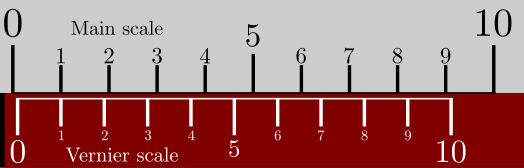
\includegraphics[width=0.95\linewidth]{figs/vernier2.png}
                \caption{Just away from 0, when the coinciding division \\is 1, the distance is $1\times\texttt{MSD}-1\times\texttt{VSD}=0.1\, \texttt{units}$.}
                \label{fig:vernier_2}
        \end{subfigure}\hfill
        \begin{subfigure}[b]{0.5\textwidth}
                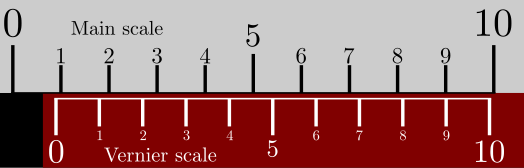
\includegraphics[width=0.95\linewidth]{figs/vernier3.png}
                \caption{Before crossing 1, the last coinciding division is 9, and the distance is $9\times\texttt{MSD}-9\times\texttt{VSD}=0.9\, \texttt{units}$.}
                \label{fig:vernier_3}
        \end{subfigure}%
        \caption{Measurement with Vernier Calipers}
        \label{fig:verniermeasurements}
\end{figure}

\begin{enumerate}
    \item Move the vernier scale \textit{slightly}, until the $1$ on the vernier scale coincides with the nearest main scale division (this is obviously the $1$ on the main scale, see Figure (\ref{fig:vernier_2})).Notice that the amount by which you have opened the jaws is the difference in size between one main-scale division and one Vernier-scale division.
    
    \item You will notice that the jaws are slightly apart. The distance between them is of course the distance the $0$ on the vernier scale has moved.
    
    \item But this distance is simply the difference between 1 Main Scale Division (\texttt{MSD}) and 1 Vernier Scale Division (\texttt{VSD}), since both the $1$ marks coincide!
    
    \item Thus, the spacing between the jaws of the calipers is now $0.1$ units!
    
    \item We have thus been able to measure a distance of $0.1$ units using two scales, one of least count $1$ unit, and the other of least count $0.9$ units! 
    
\end{enumerate}

Similarly, if you went one division further, and had the 2 of the vernier scale coincide with a main scale division, then the distance between the jaws would be $2\times\texttt{MSD}-2\times\texttt{VSD}=0.2\, \texttt{units}$. Thus, if the $n$th vernier scale division coincides with a main scale division, the distance between the jaws is $n \times (\texttt{MSD}-\texttt{VSD})=n \times \texttt{LC}$. Where \texttt{LC} is the Least Count of your Vernier calipers\footnote{In our case, the Least Count is 0.1 units.}.

Of course, up until right now we have been measuring distances between 0 and 1 unit.  What about an arbitrary distance? Consider the example given in Figure (\ref{fig:vernier_4}). 

\begin{figure}[!htb]
    \centering
    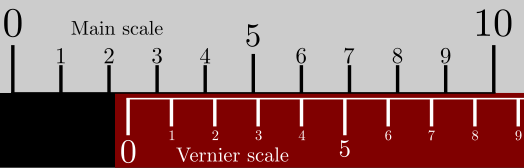
\includegraphics[scale=0.75]{figs/vernier4.png}
    \caption{The main scale reading is more than 2 units. The coinciding vernier scale division is 4 . }
    \label{fig:vernier_4}
\end{figure}

Here is the general procedure to take a reading using Vernier calipers:

\begin{enumerate}
    \item Look where the zero mark on the Vernier scale meets the main scale. This gives us our rough reading, usually called the Main Scale Reading or \texttt{MSR}. In the example in Figure (\ref{fig:vernier_4}), the \texttt{MSR} is 2.
    
    \item Now look to find the mark on the vernier scale which most closely meets any mark on the main scale. This is the Vernier Scale Reading or \texttt{VSR}, giving you the most precise digit. In this example, the \texttt{VSR} is 4.
    
    \item The total distance is given by 
    $$\texttt{distance} = \texttt{MSR} + \left(\texttt{VSR}\times\texttt{LC}\right)$$
    
    In our case, $\texttt{distance} = 0.24$ units.
    
    \item Thus, using two scales -- one of least counts $1$ unit and another of least count $0.9$ units -- we have calipers capable of measuring up to (or down to!) $0.1$ units! You have an \textit{effective least count} that is much smaller than the least count of the main scale. 
\end{enumerate}

\begin{question}
\paragraph{Question:} Show that the least count of a set of Vernier calipers is given by:
\begin{enumerate}
    \item $$\texttt{LC} = \texttt{Least count of main scale} - \texttt{Least count of vernier scale}$$
    \item $$\texttt{LC} = \frac{\texttt{Least count of main scale}}{\texttt{Number of vernier scale divisions}}$$
\end{enumerate}
\end{question}

\subsection{The Micrometer Screw Gauge}

The design of the micrometer screw gauge is different, and uses the fact that a linear movement that is imperceptible can be turned into an angular movement that is easily perceptible; the best way to understand this is simply to examine the screw gauge (which, unlike Vernier calipers, is easy to understand). The screw gauge uses a screw with an accurate and constant \textbf{pitch} (the amount by which the thimble moves forward or backward for one complete revolution) as an auxiliary scale marked on a rotatable thimble.  

The micrometers in our laboratory have a pitch of $0.01 mm$.  The rotating thimble is subdivided into 100 equal divisions.  The thimble passes through a frame that carries a millimetre scale graduated to $1 mm$.  The jaws can be adjusted by rotating the thimble using the small ratchet knob.  This includes a friction clutch which prevents too much tension from being applied.

\begin{imp}
Only tighten the screw gauge by rotating the ratchet, otherwise you may damage the instrument. Stop rotating after you hear \textbf{three} clicks. \textbf{Do not} tighten the screw any further.
\end{imp}

\begin{question}
\paragraph{Question:} Show that the least count of a screw gauge is given by
$$\texttt{LC} = \frac{\texttt{Pitch of a the screw}}{\texttt{Number of circular scale divisions}}$$
\end{question}

\section{Random Errors}

Let us go back the simple measurement of the length of an object with a ruler. We place the object against the ruler with one end flush against a certain division of the ruler, say 0 (it does not have to be 0, but usually is). Then we observe where the other end is. In general, it will be, as mentioned earlier, at some point between two successive marks on the ruler. Let us imagine doing this repeatedly. Every time we place one end against 0, it will be at \textit{slightly} different point, and so the other end will also move slightly, in a manner that we cannot control. If this movement is much smaller than the distance between two successive marks on the ruler, i.e. its least count, then this random movement will not be discernible. On the other hand, if the movement is greater than the least count of the ruler, then the length we measure will change from one measurement to the next. In the first case the error is determined by the least count of the ruler, and the length measured will not change from one measurement to the next. In the second case, however, it is clear that the length measured \text{will} change from one measurement to the next. We call this kind of error a \textit{random error}.

Another example that may make the idea clearer is the following. Imagine that a sound of a fixed duration is played over and over again, and you are required to time the duration with a stopwatch. You will have to start and stop your stopwatch over and over again. It is easy to see that even though the duration of the sound remains the same, the duration that you measure will vary from one measurement to the next. Once again we have a random error. It should be intuitively clear that the magnitude of the error depends not on the duration of the sound but on the \textit{spread} of your measurements. The number we assign to the random error must therefore be obtained from a measure of this spread. To do this, we must remove what does not matter, namely the actual duration of the sound. Generally we don't know the actual duration of the sound. So we do the best we can: we subtract the mean of our measurements from all of them, since the mean is our best guess of the actual duration. That leaves us a distribution of the variations of the measurements. 

We are not really concerned with whether the variation is positive or negative. So we use the sum of the squares of the variation, i.e. $\sum_{i = 1}^{n}(x_i - \overline{x})^2$, where $x_i$ is any reading, $\overline{x}$ is the mean, and $n$ is the total number of readings. Because the variations are both positive and negative, this sum grows not in proportion to $n$ but in proportion to $\sqrt{n}$. (This is a subtle point; you will understand it later.) So the standard measure of the spread of the readings is the standard deviation 
\begin{equation*}
    \sigma = \sqrt{\frac{\sum_{i = 1}^{n}(x_i - \overline{x})^2}{n - 1}}.
\end{equation*}

(Why $n-1$ instead of $n$ in the denominator is another subtle point. Again, let it be for the moment. Anyway, the difference between $n$ and $n-1$ is negligible for large $n$, which is the only case in which the idea of random errors is meaningful.)

\section{Errors in Time Measurements}

The time measurements you will encounter in the lab will be made by human beings (you) using clocks. If you compare the processes of measuring a duration to that of measuring a length, you will immediately see that you no longer have the luxury of aligning one end of your ``object'' (here a duration) with a physical scale: you must start your clock at a moment that you best judge to be the beginning of the duration and end it at what you best judge to be its end. Thus you automatically make two errors, one at the end of your time measurement and one at the beginning. The magnitude of the error has nothing to do with how long or short the duration is. 

Is this error due to the least count of you clock? It is -- partly; but that's not the whole story: there is another factor to take into account, your reaction time. As a human being you have to judge when when the duration begins and press the start button on your clock; both your judgement and the pressing of the button entail errors that are due to the finite time it takes for your brain and your body to react. Thus the errors at the beginning and the end of a measurement of duration are a combination of the the error due to the least count of your clock and your reaction time. If one is much larger than the other, it dominates and the other may be neglected. 

Determining the least-count error is easy: it's just the last count of your clock. Determining the error due to finite reaction time is not easy. One way is to do many measurements of a duration that is known to be constant (e.g. the period of a pendulum) and look not at the average but the spread in the readings, a measure of which is the standard deviation. For most human beings have a reaction time or about 0.1 $s$, much larger than the least count of standard lab stop watches, which is usually 0.1 $s$. Thus the error in most of your time measurements will be dominated by your reaction time. 

\subsection{Time Measurement for Periodic Phenomena}

You will often be interested in measuring a duration of a periodic phenomenon, e.g. the oscillation of a pendulum. If you assume that the period of the pendulum has a true value that does not change from one oscillation to the next, then there is a way in which you can dramatically reduce the error on the time period. Since the error in the measurement of a duration occurs only at the ends, you can simply measure the duration for many oscillations, e.g. 10 or 100, and divide by that number. So, if the total error due to your reaction time on a duration (i.e at both ends of a duration together) is 0.1 $s$ and you measure the duration for 10 oscillations, the error associated with a single time period will be $0.1/10 = 0.01 s$.

Given that this is true, you may ask why one doesn't simply measure the duration for 1000 oscillations (or some arbitrarily large number). One answer is that the oscillations will damp out. The other had to do with human fatigue: if you are asked to count 1000 oscillations, you may make an error in counting the number of oscillations, and that would lead a much larger loss in precision than what you gained by increasing the number of oscillations. (Machines don't have this problem and it makes sense, when a mechanical counter is being used, to increase the number of oscillations as much as possible.) 

A question that might arise is what happens if we measure the duration for 10 oscillations several times. Is this equivalent to measuring the duration for 100 oscillations? No. Now we have a pair of end points for each duration of 10 oscillations, and each point is associated with starting and stopping a clock. If we measure the duration for 100 oscillations (let us call this case 1), we have 2 end points, and if we measure 10 sets of 10 oscillations each (case 2), we have 20 end points, i.e. there are 10 times as many points at which errors can occur. From this we may at first conclude that the error in case 2 is 10 times the error is case 1, but that is not correct: the errors we make at the end points can be either overestimates of underestimates, i.e. positive or negative, and so as we stack up the end points there will be some cancellation. It an be shown -- and at some point you will show this -- that as the number of end points $n$ increases, the error goes up as $\sqrt{n}$. Thus, if the error on time measurement with single pair of end points is $\Delta t$, the error on combining $n$ time measurements is $\sqrt{n} \, \Delta t$. Putting all this together, if the error on a single time measurement is $\Delta t$, the error on the time period $T$ using 100 oscillations is $\frac{\Delta t}{n}$ and the error on $T$ using 10 measurements of 10 oscillations each is $\frac{\sqrt{n} \, \Delta t}{n} = \frac{\Delta t}{\sqrt{n}}$. (Don't worry if this paragraph went over your head; you will understand it slowly, over the semester.)

It should be obvious the from the discussion above that while time measurement is much more subtle than length measurement it allows an almost arbitrary improvement in precision (reduction in error) on the time period itself (to be distinguished from the duration of a measurement)  if the phenomenon is periodic. This can be used to great effect in certain devices, e.g. the Kater's pendulum. To ensure that this great advantage is not vitiated by incorrect counting of oscillations, it is very important to know exactly how to count the number of oscillations. A very common error is to count $n-1$ oscillations when one wants to count $n$. You will learn the correct procedure in the lab. 

%\section{Theory: Error Analysis}

%\subsection{Types of Errors}

%``Error'' analysis is a rather glaring misnomer. All measurements have some degree of uncertainty that may come from a variety of sources, from the lack of precision of the measuring instrument to random fluctuations in the environment. The process of evaluating the uncertainty associated with a measurement result is often called uncertainty analysis or error analysis. However, the common definition of an ``error'' being a ``mistake'' is very misleading. However, the terminology is so rampant that we will be forced to use it at times, referring to `error' analysis when we really mean `uncertainty' analysis.


\begin{tip}
\paragraph{A cautionary tale:} Neutrinos are weakly interacting nearly massless particles that are theorised to be moving close to -- if not at -- the speed of light.\\

In September 2011, scientists of the OPERA collaboration reported evidence that neutrinos they produced at CERN in Geneva and recorded at the OPERA detector at Gran Sasso, Italy, had travelled \textbf{faster} than light. If this were true, it would have violated one of the pillars of modern physics, the Theory of Relativity.\\

The neutrinos were calculated to have arrived approximately 60.7 nanoseconds sooner than light would have if it had traversed the same distance in a vacuum. Assuming the error were entirely due to random effects, scientists calculated that there was a 0.2-in-a-million chance that this may be a false positive.\\

In March 2012 it was confirmed that a fibre cable was not fully screwed in during data gathering, and this effectively decreased the reported flight time of the neutrinos by 73ns, making them seem faster than light. The corrected difference between the measured and expected arrival time of neutrinos (compared to the speed of light) was approximately 6.5 $\pm$ 15 ns. This is consistent with \textbf{no difference at all}, thus the speed of neutrinos is consistent with the speed of light within the margin of error.
\end{tip}

%\subsubsection{Least count errors}

%As you have already seen, the least count of a measuring instrument is the smallest value the instrument can resolve. For example, if we use a metre scale to measure an object and find that it is $23.5$cm, the uncertainty here \textbf{due to the measuring instrument} is $0.1$cm. Thus, we can say that the length of the object is given by $l = (23.5 \pm 0.1) cm$ where $\pm \Delta l = \pm 0.1$cm is the uncertainty in measurement due to the least count of the metre scale. This is the value up to which the `best' value of $23.5$ may be specified with any confidence.

%In general, such errors are the \textbf{lower bounds} of experimental errors. No error that is less than the least count error need be considered. That being said, if you find other sources of error to be greater than the least count error, then those sources should be used. For example, the stopwatches in the lab have a least count of $0.01$s. However, your reaction time of turning on and off a stopwatch would be at best $0.1$s. Thus, while the least count error is significantly smaller, the \textbf{actual} error in a time measurement using the stopwatch would be of the order of $0.1$s.

%\subsubsection{Systematic errors}

%Imagine now that the metre scale that you are using to measure the length of the object is made of metal, and as a result expands slightly in summer. If you performed a set of measurements, you would obviously not find the `true' value of the length. However, such an error may be discovered by comparing your measurements from the metal scale with a wooden scale, for example. When using instruments like digital multimeters you obviously rely on it having been calibrated properly. However, there might have been an accident that a student did not report, and as a result there could well be a systematic error for someone unlucky enough to be the one using it next.

%\subsubsection{Random errors}

%Another reason for two measurements not agreeing totally is due to small, uncorrelated variations in the environment or measurement process. For example, while measuring the time period of a pendulum, you might get different readings due to small differences in your reaction time. Similarly, when measuring the height of a cylinder with a vernier calliper, you may see small variations depending on \textbf{where} you measure the height, as it is possible the cylinder was not made to be smooth up to $0.1$mm everywhere.

%Such variations, being \textbf{random}, are expected to fall just as often \textit{above} a certain value as \textit{below} it. A truly random source would give you a \textbf{Gaussian} distribution of errors; the mean of this distribution $$\overline{m}_N = \frac{\sum_{i=1}^{N}{m_i}}{N}$$ would approach the `best' value as the number $N$ of well-sampled values increases. The uncertainty of these measurements would then be quantified by the \textbf{standard deviation}\footnote{There is a reason for the $N-1$, it is known as the number of `degrees of freedom' in statistics. Understanding it is not essential for this course.} $$\Delta m_N = \sqrt{\frac{(m_i - \overline{m}_N)^2}{N-1}}$$

%more conventionally denoted by $\sigma$.

\subsubsection{Precision, Accuracy, and Statistics}

\begin{enumerate}
    \item \textbf{Accuracy:} is how closely a measurement comes to some `true' value. It determines how well we have eliminated \textbf{\textit{systematic errors}} and mistakes in our measurements.
    \item \textbf{Precision:} is how closely a set of measurements agree \textit{with each other}. %It determines how well we have eliminated \textbf{\textit{random errors}} in our measurements.
\end{enumerate}

To use a sports simile, if you're playing football and are accurate, your aim will always take the ball close to or into the goal. If, however, you harbour a personal grudge against the coach and succeed in beaning him on the head every time you get the ball, then you would be \textit{precise}, but not accurate.\footnote{It is widely accepted that the point of football get the ball into the goal and not to traumatise your coach, which is why this example works.}

\textbf{A caveat:} In any physics experiment worth doing, you usually don't have the answer beforehand. This means you don't have a ``true'' value with which to compare your answer. This is why it is so important to be both precise (reduce all random errors present in your measurements) and accurate (reduce all systematic errors present in your measurement). You must also, however, come up with ways to check if your answer is accurate \textit{without} trying to resort to a ``textbook'' solution.

\begin{question}
\paragraph{Question:} In the example of the `superluminal' neutrinos given earlier, was the error of the OPERA team one of inaccuracy, or of imprecision? 
\end{question}

\section{Propagation of Errors}

In general we are interested not just in our observations but in quantities derived from them, i.e. in derived quantities. It is obvious that the a derived quantity will inherit some the errors in the observations from which it is derived. But to what extent will it do so? We will use a few examples to understand this. 

\begin{enumerate}
    \item We want the radius of a diameter, we usually measure its diameter. Here the observed quantity is the diameter $d$ and the derived quantity is the the radius $r$. We have $r = d/2$. Thus if there is an error of $\pm \delta$ in measuring $d$ (for example due to the least count of the measuring instrument), then, clearly the error in $r$ is $\pm \delta/2$.
    
    \item We want the perimeter $p$ of a rectangle having measured its length $l$ and its width $w$. $p = 2l + 2w$. If the errors in measuring $l$ and $w$ are $\pm \delta$, for each, the error in $p$ is clearly $\pm 2 \delta \pm 2 \delta$, which ranges between $- 4 \delta$ and $+ 4\delta $, depending on the signs on the errors on $l$ and $w$. So the error on $p$ is $\pm 4 \delta$.
    
    \item We want the area $A$ of a rectangle having measured its length $l$ and its width $w$. $A_\text{true} = l \, w$. Suppose that the error in the measurement of $l$ is $\pm \delta l$ and the error in measuring $w$ is $\delta w$, then what we derive is $A_\text{derived} = (l \pm \delta l) (w \pm \delta w)$. If the errors are much smaller than measurements, we can neglect terms of order $\delta^2$. Then, the value of $A_\text{derived}$ ranges between $A_\text{true} - w \delta l - l \delta w$ and $A_\text{true} +  w \delta l + l \delta w$. Notice that the expression for the error is rather complicated; we can simplify it if we express it in terms of the relative error. Since the error in $A$ is $\delta A = A_\text{derived} - A_\text{true}$, you can easily show that 
    \begin{equation*}
        \frac{\delta A}{A} = \pm \frac{\delta l}{l} \pm \frac{\delta w}{w}.
    \end{equation*}
    The quantity $\delta x / x$ is called the \textit{relative error} in $x$.
    
    \item We want the volume $V$ of a sphere given a measurement of its diameter $d$. You can easily show, using the method given above, that 
\begin{equation*}
    \frac{\delta V}{V} = \pm 3 \, \frac{\delta d}{d}.
\end{equation*}
Notice how the sensitivity of the relative error in $V$ to the relative error in $d$ depends on the \textit{power} in the dependence of $V$ on $d$. (Since $V = (4/3) \pi r^3$, $V \propto d^3$.
    
    \item We want the mass per unit length $\lambda$ of a wire having measured its mass $m$ and its length $l$, with . $\lambda_\text{true} = (m \pm \delta m) / (l \pm \delta l)$. If you go through the same process as in the last case considered, you will find that 
    \begin{equation*}
        \frac{\delta \lambda}{\lambda} = \pm \frac{\delta m}{m} \pm \left( -\frac{\delta l}{l} \right).
    \end{equation*}
    
\end{enumerate}

\section{Using Error Analysis to Plan Your Experiment}

Suppose that you want to measure the volume of a tile (whose length $l$ and width $w$ are much greater than its thickness $t$). Since $V = l \times w \times t$, you have
\begin{equation*}
    \frac{\delta V}{V} = \pm \frac{\delta l}{l} \pm \frac{\delta w}{w} \pm \frac{\delta h}{h}.
\end{equation*}
This formula shows you right away that there is not much point improving one measurement indefinitely if the dominant cause of error is another measurement. What we want is for all the measurements to contribute more or less equally. This immediately tells us that we must choose our instruments so that this goal is achieved. 

\begin{question}
\paragraph{Question:} What instruments would you choose measure the length, width, and thickness of the tile so that the relative errors in them are comparable?~\\

%\vspace{0.5 cm}

\paragraph{Question:} Suppose $P = x y^3$, where $x$ and $y$ are the measured quantities. On which of them is the relative error in $P$ more sensitive?

\end{question}

\section{The Experiment}

\subsection{Apparatus}

\begin{enumerate}
    \item A pair of Vernier calipers
    \item A Screw gauge
    \item A set of ball bearings
    \item A set of aluminium cylinders
    \item A small measuring flask
    \item A container with a spout
\end{enumerate}

\subsection{Description}

\begin{enumerate}
    \item In \textbf{Part A} you will measure the radius, height, and volume of different cylinders. You will then plot an appropriate graph from which you will extract the value of $\pi$.
    
    \item In \textbf{Part B} you will measure the radius and volume of different ball bearings. You will then plot an appropriate graph from which you will extract the value of $\pi$.
    
\end{enumerate}

\subsection{Suggested Procedure}

\subsubsection{Part A}

\begin{enumerate}
    \item Decide on the best instrument and method to measure the following properties of the cylinders:
    \begin{enumerate}
        \item Radius
        \item Height
        \item Volume
    \end{enumerate}
    
    \begin{question}
        \paragraph{Question:} How and where would you measure the radius of the cylinders? How many trials would you take?
    \end{question}
    
    \item Be sure to take a sufficient number of \textbf{well-sampled} readings.
    
    \item Decide on an appropriate graph between the measured quantities from which you can extract the numerical value of $\pi$.
\end{enumerate}

\subsubsection{Part B}

\begin{enumerate}
    \item Decide on the best instrument and method to measure the radii and the volumes of the bearings.
    
    \item Be sure to take a sufficient number of \textbf{well-sampled} readings.
    
    \item Decide on an appropriate graph between the measured quantities to extract the numerical value of $\pi$.
\end{enumerate}

\begin{question}
\paragraph{Question:} How does your estimate compare with the known value of $\pi \approx 3.14159$?
\end{question}



\newpage